\documentclass[cjk,slidestop,compress,mathserif,blue]{beamer}
%dvipdfm选项是关键,否则编译统统通不过
%beamer的颜色选项定义的是导航条和标题的颜色(即关键词structure的颜色)

%%%%%%%%%%%%%%%%仅限于XeTeX可使用的宏包%%%%%%%%%%%%%%%%%%%%%%%%%%%%
\usepackage{fontspec,xunicode,xltxtra,beamerthemesplit}
%\usepackage{beamerthemesplit}
\usepackage{xeCJK}
\setCJKmainfont[BoldFont=黑体, ItalicFont=楷体, BoldItalicFont=仿宋]{黑体}
%\setsansfont[Mapping=tex-text]{Adobe 黑体 Std}
%如果装了Adobe Acrobat,可在font.conf中配置Adobe字体的路径以使用其中文字体
%也可直接使用系统中的中文字体如SimSun,SimHei,微软雅黑 等
%原来beamer用的字体是sans family;注意Mapping的大小写,不能写错

%%%%%%%%   确定标题和导航条结构的框架     %%%%%%%%%%%%
\usepackage{beamerthemeshadow}                       %
%\usepackage{beamerthemeclassic}%导航条色与背景色一致%
%%%%%%%%%%%%%%%%%%%%%%%%%%%%%%%%%%%%%%%%%%%%%%%%%%%%%%
\setbeamerfont{roman title}{size={}}
%\usepackage{CJK} % CJK 中文支持                                  %
\usepackage{amsmath,amsthm,amsfonts,amssymb,bm}
\usepackage{bbding}
\usepackage{mathrsfs}
\usepackage{xcolor}                                        %使用默认允许使用颜色
\usepackage{hyperref} 
\usepackage{graphicx}
\usepackage{subfigure}           %图片跨页
\usepackage{animate}		 %插入动画
\usepackage{caption}
\captionsetup{font=footnotesize}

%\usepackage[version=3]{mhchem}		%化学公式
\usepackage{chemformula}
\usepackage{chemfig}		%化学公式

\usepackage{multirow}
\usepackage{makecell}		%允许单元格内换行

\usepackage[dvipdfmx]{movie15_dvipdfmx} %插入视频
%\usepackage{handoutWithNotes}		%(讲义)在打印PPT的时候会留出给每一页做注释的部分
%\pgfpagesuselayout{1 on 1 with notes landscape}[a4paper,border shrink=5mm]

%\usepackage[numbers,sort&compress]{natbib} %紧密排列             %
\usepackage[sectionbib]{chapterbib}        %每章节单独参考文献   %
\usepackage{hypernat}                                                                         %
%\usepackage[dvipdfm,bookmarksopen=true,pdfstartview=FitH,CJKbookmarks]{hyperref}		%
\hypersetup{bookmarksnumbered,colorlinks,linkcolor=brown,citecolor=blue,urlcolor=red}         %
%参考文献含有超链接引用时需要下列宏包,注意与natbib有冲突        %
%\usepackage[dvipdfm]{hyperref}                                  %
%\usepackage{hypernat}                                           %
\newcommand{\upcite}[1]{\hspace{0ex}\textsuperscript{\cite{#1}}} %

%\useoutertheme{smoothbars}
\useinnertheme[shadow=true]{rounded}
\usetheme{Berkeley}                                          %主题式样
%\usetheme{Luebeck}

\usecolortheme{lily}                                        %颜色主题式样

\usefonttheme{professionalfonts}                           %字体主题样式宏包

%\beamertemplatetransparentcoveredhigh                      %使所有被隐藏的文本高度透明
\beamertemplatetransparentcovereddynamicmedium             %使所有被隐藏的文本完全透明,动态,动态的范围很小
\mode<presentation>
%\beamersetaveragebackground{gray}                          %设置背景颜色(单一色) 
\beamertemplateshadingbackground{green!10}{red!5}         %设置背景颜色(渐变色)

%在指定位置精确放置logo
\usepackage{tikz}
\usepackage{beamerfoils}
\usepackage{pgf}
\logo{\pgfputat{\pgfxy(9.99,0.00)}{
\includegraphics[height=0.75cm,viewport=5 2 520 120,clip]{Figures/BCC_logo-1.png}}}
%\logo{\pgfputat{\pgfxy(10.45,0.00)}{
\includegraphics[height=0.65cm,viewport=6.5 39 264 102,clip]{Figures/BCC_logo-2.jpg}}}
%\logo{\pgfputat{\pgfxy(11.68,0.15)}{
\includegraphics[height=1.01cm,viewport=0 0 140 120,clip]{Figures/BCC_logo-1.png}}\pgfputat{\pgfxy(10.502,-0.218)}{
\includegraphics[height=0.369cm,viewport=140 0 540 120,clip]{Figures/BCC_logo-1.png}}}
%\logo{\pgfputat{\pgfxy(11.38,0.24)}{
\includegraphics[height=1.50cm,viewport=26 12 440 420,clip]{Figures/BCC_logo.jpg}}}

%\logo{\pgfputat{\pgfxy(10.28,0.00)}{
\includegraphics[height=0.95cm,viewport=0 0 1100 360,clip]{Figures/Logo_Gainstrong.png}}}
%\logo{\pgfputat{\pgfxy(11.68,0.15)}{
\includegraphics[height=0.95cm,viewport=0 0 510 360,clip]{Figures/Logo_Gainstrong.png}}\pgfputat{\pgfxy(10.333,-0.195)}{
\includegraphics[height=0.35cm,viewport=530 70 1100 218,clip]{Figures/Logo_Gainstrong.png}}}
%\MyLogo{
%	\pgfputat{\pgfxy(-50,-50)}{\pgfbox[right,base]{
\includegraphics[height=1cm]{Figures/BCC_logo-1.png}}}

%logo作为背景放置
%\setbeamertemplate{background}{
%	\pgfputat{\pgfxy(6.5,-0.5)}{\pgfbox[left,top]{\pgfimage[height=1.1cm]{Figures/BCC_logo-1.png}}}}

%\logo{}									%不显示logo

\begin{document}
%\begin{CJK*}{GBK}{song}
%\begin{CJK*}{GBK}{kai}
%beamer下不能用\songyi、\zihao等命令!
%\graphicspath{Figures/}

%-------------------------------PPT Title-------------------------------------
\title{面向甲烷燃烧机理研究的\\异质界面催化模拟自动流程软件开发}
%-----------------------------------------------------------------------------

%----------------------------Author & Date------------------------------------
\author[]{北京市计算中心\;云平台\:姜骏}
	
\institute[]{}
%\date{2013.09.10}
\date{\textrm{2020.11.19}}
\frame
{	
	\frametitle{\footnotesize{\textcolor{orange}{\textrm{2018~}年度“青年骨干计划”答辩}}}
\titlepage
}
%-----------------------------------------------------------------------------

%------------------------------------------------------------------------------列出全文 outline ---------------------------------------------------------------------------------
\section*{}
\frame[allowframebreaks]
{
  \frametitle{Outline}
%  \frametitle{\textcolor{mycolor}{\secname}}
  \tableofcontents%[current,currentsection,currentsubsection]
}
%在每个section之前列出全部Outline
%类似的在每个subsection之前列出全部Outline是\AtBeginSubsection[]
\AtBeginSection[]
{
  \frame<handout:0>
  {
    \frametitle{Outline}
%全部Outline中,本部分加亮
    \tableofcontents[current,currentsection]
  }
}

%------------------------------------------------------------------------------PPT main Body------------------------------------------------------------------------------------
\small
%\section{个人信息}
\frame
{
	\frametitle{个人信息}
	\vskip -45pt
\begin{minipage}[b]{0.72\linewidth}
	\fontsize{9.2pt}{6.2pt}\selectfont{姓~名\hspace{15pt}姜~骏\hspace{45pt}出生年月\hspace{15pt}\textrm{1978.12}}\\
	\vskip 7pt
	学~位\hspace{15pt}理学博士\hspace{29pt}专业方向\hspace{15pt}物理化学\\
	\vskip 7pt
	\fontsize{8.2pt}{6.2pt}\selectfont{工作部门\hspace{5pt}北京市计算中心~云平台事业部}\\
\end{minipage}
\hfill
\begin{minipage}[b]{0.26\linewidth}
	\vspace{40pt}
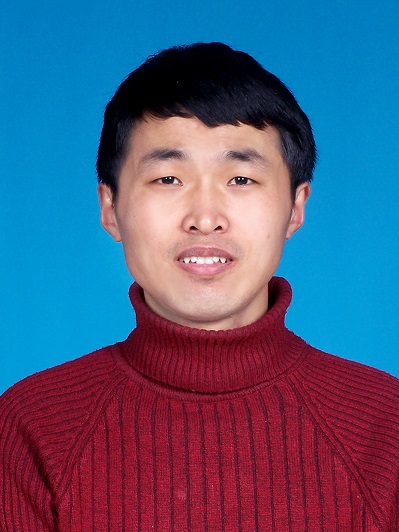
\includegraphics[height=0.7in]{Figures/Person_Photo.JPG}\\
\end{minipage}\vskip 3pt
\fontsize{9.2pt}{6.2pt}\selectfont{\textcolor{magenta}{教育背景}}
	\begin{itemize}
		\item {\fontsize{8.2pt}{6.2pt}\selectfont{\textrm{2001.09-2008.01}}}~~~北京大学~化学与分子工程学院~~~~~~物理化学
		\item {\fontsize{8.2pt}{6.2pt}\selectfont{\textrm{1997.09-2001.06}}}~{\fontsize{8.2pt}{6.2pt}\selectfont{中国纺织大学(现~东华大学)}}~{\fontsize{8.2pt}{6.2pt}\selectfont{纺织化学系~染整工程}}
	\end{itemize}
	\fontsize{9.2pt}{6.2pt}\selectfont{\textcolor{magenta}{工作简历}}
\begin{table}[!h]
\tabcolsep 0pt \vspace*{-5pt}
%\caption{经费预算表 (单位:~万元).}
\label{Table-Cost}
%\begin{minipage}{\textwidth}
%\begin{center}
\centering
\def\temptablewidth{0.94\textwidth}
\renewcommand\arraystretch{2.2} %表格宽度控制(普通表格宽度的两倍)
\rule{\temptablewidth}{1pt}
\begin{tabular*} {\temptablewidth}{@{\extracolsep{\fill}}c@{\extracolsep{\fill}}c@{\extracolsep{\fill}}c}
%-------------------------------------------------------------------------------------------------------------------------
	起止时间 &工作单位	&研发岗位 \\\hline
	\fontsize{8.2pt}{6.2pt}\selectfont{\textrm{2008.01-2012.03}} &\fontsize{8.2pt}{6.2pt}\selectfont{北京大学~化学与分子工程学院} &\fontsize{8.2pt}{6.2pt}\selectfont{博士后(两期)} \\
	\fontsize{8.2pt}{6.2pt}\selectfont{\textrm{2012.03-2013.03}} &\fontsize{8.2pt}{6.2pt}\selectfont{北京宏剑公司} \fontsize{8.2pt}{6.2pt}\selectfont{&高级技术支持}\\
	\fontsize{8.2pt}{6.2pt}\selectfont{\textrm{2013.04-2016.03}} &\fontsize{7.8pt}{6.2pt}\selectfont{中物院高性能数值模拟软件中心} &\fontsize{8.2pt}{6.2pt}\selectfont{金属材料模拟团队} \\
	\fontsize{8.2pt}{6.2pt}\selectfont{\textrm{2016.04-至今}}    &\fontsize{8.2pt}{6.2pt}\selectfont{北京市计算中心} &\fontsize{8.2pt}{6.2pt}\selectfont{云平台事业部}
\end{tabular*}
\rule{\temptablewidth}{1pt}
%\end{center}
%\end{minipage}
\end{table}
%\vskip -3pt
}

\section{项目背景}
\frame
{
	\frametitle{项目背景}
	\begin{itemize}
		\item 天然气储量丰富、热效率高、价格低廉、污染较小。但天然气主要成分甲烷直接燃烧,温度高达~1600$^{\circ}\mathrm{C}$左右,在没有催化剂的情况下,在空气中燃烧生成氮氧化物等物质,对环境造成一定的污染。通过催化剂作用,降低燃料的起燃温度和燃烧的峰值温度,提高甲烷燃烧利用率,减少大气污染物生成
	\end{itemize}
\begin{figure}[t!]
\centering
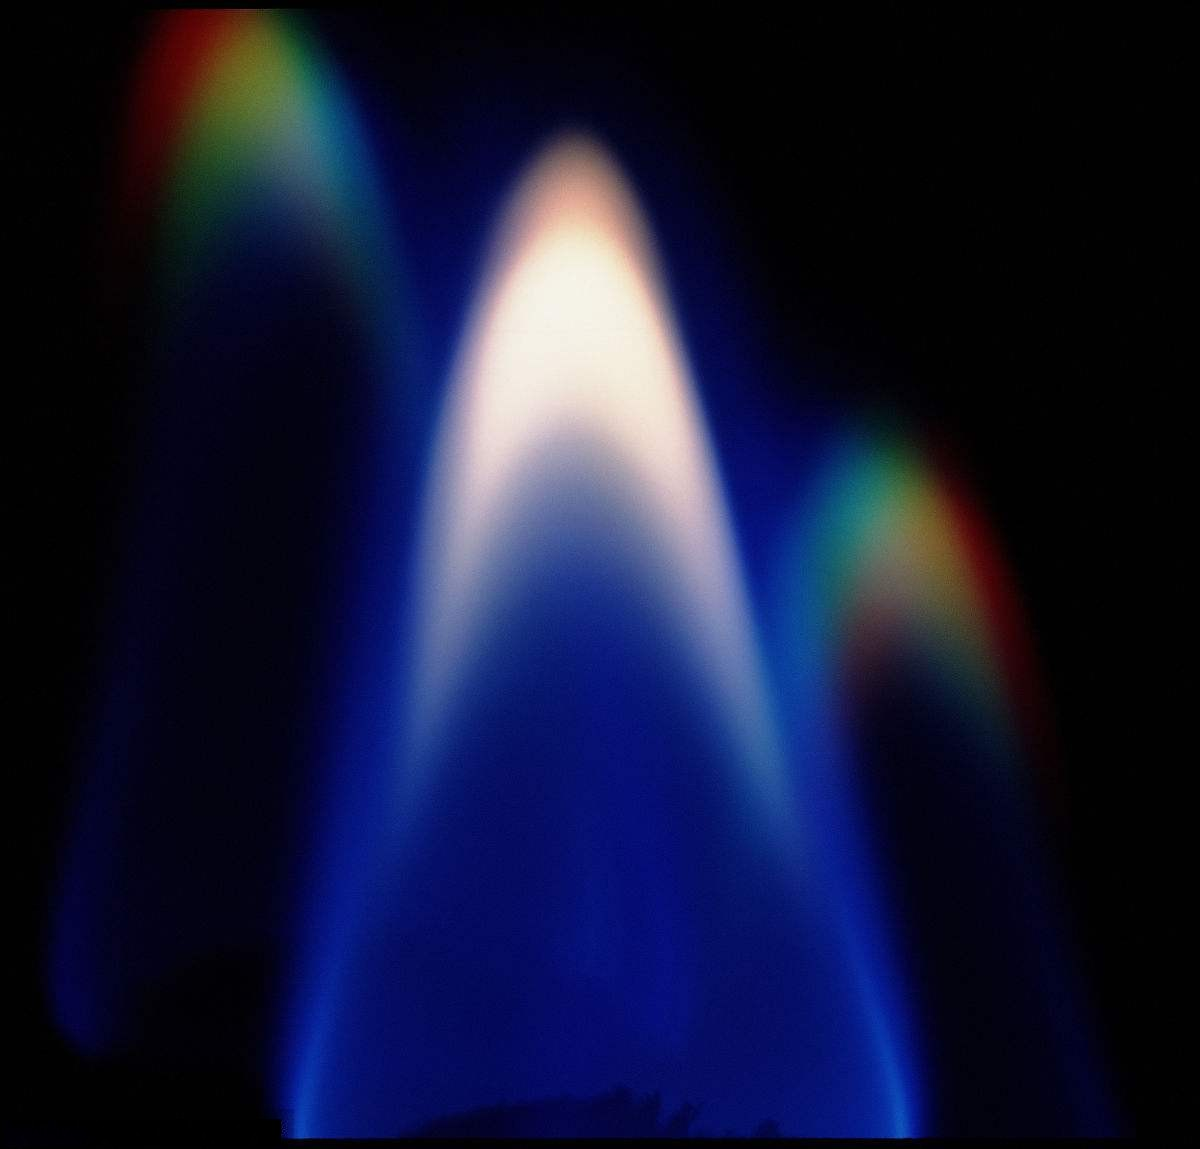
\includegraphics[height=1.3in]{Figures/CH4_combustion.jpg}
\label{fig:Combusrion_CH4}
\caption{\footnotesize \textrm{The combustion of \ch{CH4}}.}%
\end{figure} 
}

\section{项目概况}
\subsection{项目目标}
\frame
{
	\frametitle{项目目标}
\begin{minipage}[b]{0.58\linewidth}
	\begin{itemize}
		\setlength{\itemsep}{15pt}
		\item 针对第一原理计算特点,开发适应甲烷催化燃烧机理研究的自动流程计算平台并程序化
		\item 自动流程计算平台将包括结构建模的可视化,计算流程的自动化,结果数据分析的可视化
		\item 将开发的自动流程应用于甲烷燃烧催化剂计算%六铝酸盐系列(\chemfig{MAl_{12}O_{19}})
	\end{itemize}
\end{minipage}
\hfill
\begin{minipage}[b]{0.38\linewidth}
\begin{figure}[t!]
\centering
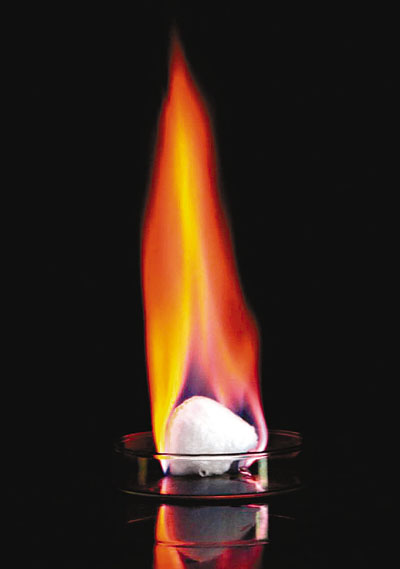
\includegraphics[height=1.3in]{Figures/combustible_ice.jpg}
\label{fig:Combustible_ice}
%\caption{\footnotesize \textrm{The Structure of \chemfig{MAl_{12}O_{19}}.}}%
\caption{\footnotesize \textrm{Combustion of the Flammable ice.}}%
\end{figure} 
\end{minipage}
}

%\section{高通量材料计算自动流程软件开发}
\frame
{
	\frametitle{跨尺度材料模拟自动流程软件现状}
\begin{itemize}
	\setlength{\itemsep}{1pt}
	\item {\fontsize{8.2pt}{4.2pt}\selectfont{\textcolor{purple}{高温合金材料}:~微观原子间相互作用决定体系的宏观力学性质}}
	\item {\fontsize{8.0pt}{4.2pt}\selectfont{\textcolor{purple}{催化活性材料}:~与反应物间相互作用强弱,直接影响材料的催化性能}}
\end{itemize}

\begin{minipage}[b]{1.0\linewidth}
%	\begin{itemize}
%		\item \fontsize{8.0pt}{4.2pt}\selectfont{国内外现有自动流程软件概况}
%	\end{itemize}
\begin{table}[!h]
\tabcolsep 0pt \vspace*{-5pt}
\caption{\fontsize{8.0pt}{4.2pt}\selectfont{国内外现有自动流程软件概况}}
\label{Table-Cost}
\vskip -12pt
%\begin{center}
\centering
\def\temptablewidth{0.9\textwidth}
\renewcommand\arraystretch{0.8} %表格宽度控制(普通表格宽度的两倍)
\rule{\temptablewidth}{1pt}
\begin{tabular*} {\temptablewidth}{@{\extracolsep{\fill}}c@{\extracolsep{\fill}}c@{\extracolsep{\fill}}c@{\extracolsep{\fill}}c@{\extracolsep{\fill}}c@{\extracolsep{\fill}}c@{\extracolsep{\fill}}c}
%-------------------------------------------------------------------------------------------------------------------------
	&\multirow{2}{*}{\fontsize{5.2pt}{4.2pt}\selectfont{编程语言}}	&\fontsize{5.2pt}{4.2pt}\selectfont{建模} &\multicolumn{2}{|c|}{\fontsize{4.2pt}{3.2pt}\selectfont{任务提交与管理}} &\multirow{2}{*}{\fontsize{5.2pt}{4.2pt}\selectfont{后处理}} &\multirow{2}{*}{\fontsize{4.2pt}{3.2pt}\selectfont{数据组织管理}} \\\cline{4-5}
	&	&\fontsize{5.2pt}{4.2pt}\selectfont{功能} &\multicolumn{1}{|c|}{\fontsize{5.2pt}{4.2pt}\selectfont{~~~~软件接口~~~~}} &\multicolumn{1}{c|}{\fontsize{5.2pt}{4.2pt}\selectfont{运行容错~~~~~~~}} & & \\\hline
	\fontsize{5.2pt}{4.2pt}\selectfont{{AFLOW}} &\fontsize{5.2pt}{4.2pt}\selectfont{C++} &\checkmark &\triangle &\FiveStarOpen &\FiveStarOpen &\fontsize{5.2pt}{4.2pt}\selectfont{{Django}} \\
	\fontsize{5.2pt}{4.2pt}\selectfont{{MP}} &\fontsize{5.2pt}{4.2pt}\selectfont{Python} &\checkmark &\checkmark &\FiveStarOpen &\FiveStarOpen &\fontsize{5.2pt}{4.2pt}\selectfont{{MongoDB}} \\
	\multirow{2}{*}{\fontsize{5.2pt}{4.2pt}\selectfont{{QMIP}}} &\fontsize{5.2pt}{4.2pt}\selectfont{JavaScript/SVG} &\multirow{2}{*}{\checkmark} &\multirow{2}{*}{\checkmark} &\multirow{2}{*}{--} &\multirow{2}{*}{\checkmark} &\multirow{2}{*}{--} \\
	&\fontsize{5.2pt}{4.2pt}\selectfont{+html/Python} & & & & & \\
	\fontsize{5.2pt}{4.2pt}\selectfont{{CEP}} &\fontsize{5.2pt}{4.2pt}\selectfont{Python} &\checkmark &\checkmark &-- &\checkmark &\fontsize{5.2pt}{4.2pt}\selectfont{{Django/MySQL}} \\
	\fontsize{5.2pt}{4.2pt}\selectfont{{ASE}} &\fontsize{5.2pt}{4.2pt}\selectfont{Python} &\FiveStarOpen &\FiveStarOpen &-- &\triangle &-- \\
	\multirow{2}{*}{\fontsize{5.2pt}{4.2pt}\selectfont{{MatCloud}}} &\fontsize{5.2pt}{4.2pt}\selectfont{JavaScript} &\multirow{2}{*}{\checkmark} &\multirow{2}{*}{\triangle} &\multirow{2}{*}{\checkmark} &\multirow{2}{*}{\checkmark} &\multirow{2}{*}{\fontsize{5.2pt}{4.2pt}\selectfont{{MongoDB}}} \\
	&\fontsize{5.2pt}{4.2pt}\selectfont{+.NETCore} & & & & &
\end{tabular*}
\rule{\temptablewidth}{1pt}
%\vskip -15pt
%\end{center}
\end{table}
%\begin{description}
%	\item[\FiveStarOpen]~该功能较突出
%	\item[\checkmark]~该功能基本满足需求
%	\item[\triangle]~该功能存在不足
%\end{description}
\fontsize{6.2pt}{3.2pt}\selectfont{
~~~~~~~~\FiveStarOpen~表示该功能较突出;~\checkmark~表示该功能基本满足需求;~$\triangle$~表示该功能存在不足
}
\end{minipage}
}

\subsection{软件开发}
\frame
{
	\frametitle{适应异质界面催化模拟自动流程软件开发}
\begin{minipage}[b]{0.47\linewidth}
	\begin{itemize}
		\item \fontsize{8.0pt}{4.2pt}\selectfont{适用于异质界面的高通量材料计算自动流程软件架构}
\begin{figure}[h!]
\centering
\hskip -35pt
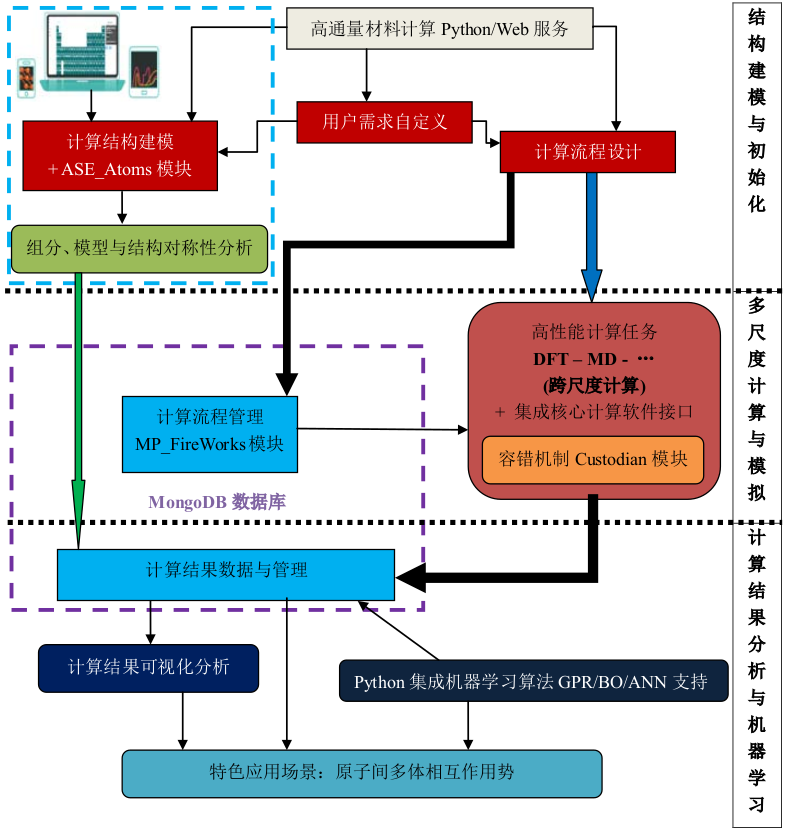
\includegraphics[height=2.18in]{Figures/MP_comp_BCC.png}
%\caption{\fontsize{6.5pt}{4.2pt}\selectfont{适应多体相互作用的高通量计算流程结构示意}}%
\label{MP_comp_BCC}
\end{figure}
	\end{itemize}
\end{minipage}
~
\begin{minipage}[b]{0.42\linewidth}
\begin{itemize}
	\item “标准化”对称性分析功能:~降低\textrm{DFT}的计算量
	\item \textcolor{magenta}{$\vec k\cdot\vec p$方法}:~提升电子计算的规模%,为\textrm{DFT-MD}计算提供基础
	\item \textcolor{magenta}{机器学习}:~优化电子计算结果,获得\textrm{MD}尺度力场,\textrm{DFT-MD}耦合%,获得\textrm{MD}尺度下准确的多体相互作用的力场函数。
	\item 设计合理完善的程序流程:~利用\textrm{MongoDB}支持的\textrm{FireWorks}计算流程管理%,由微观尺度\textrm{DFT}计算获得介观或宏观尺度的计算物性或者使不同尺度的计算结果更好地实现耦合自洽
\end{itemize}
\end{minipage}
}

\frame
{
	\frametitle{对称性分析:~空间群对称性与能带}
\begin{minipage}[b]{0.46\linewidth}
\begin{figure}[h!]
\centering
\vspace*{-0.2in}
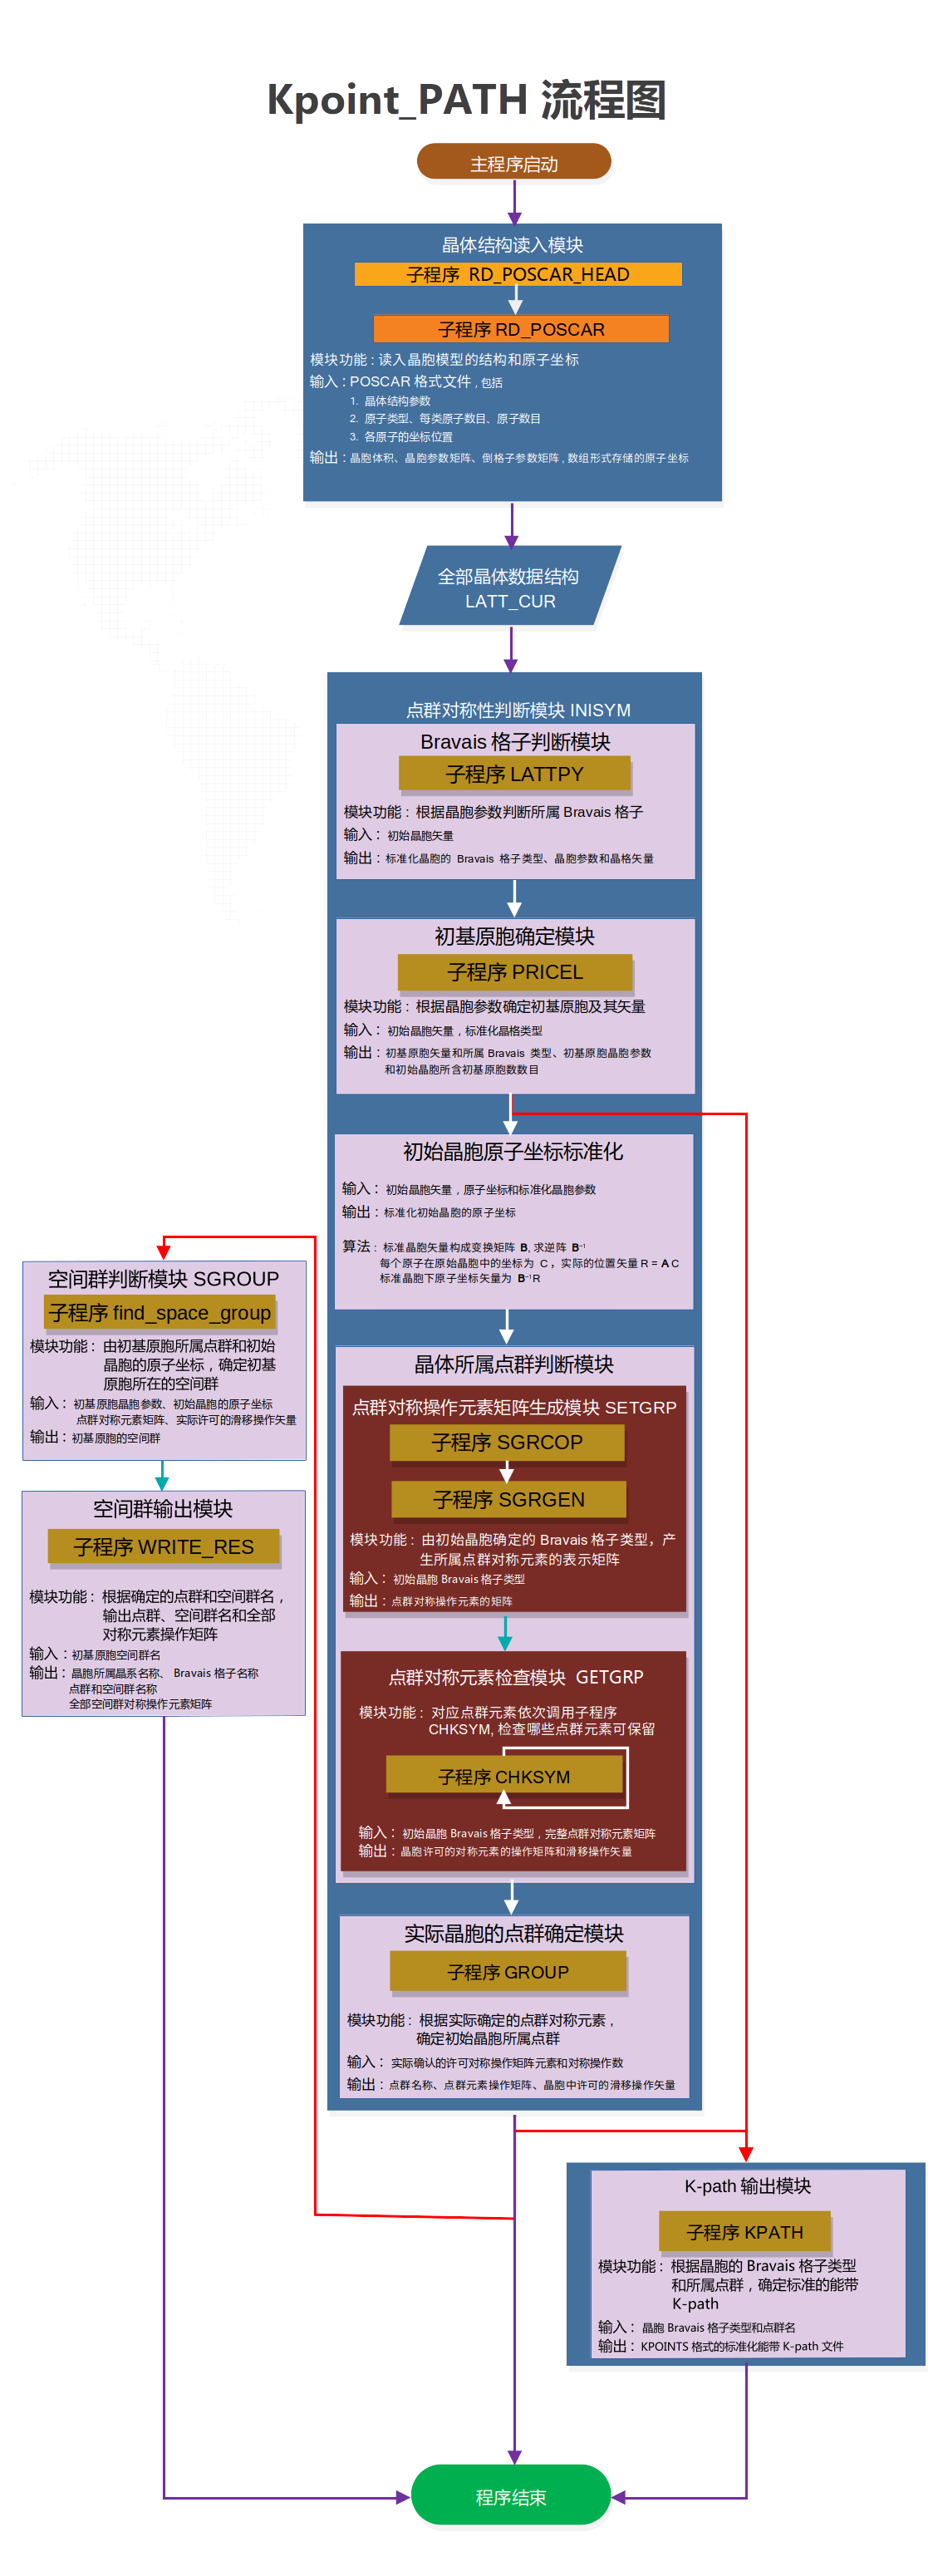
\includegraphics[height=3.05in,width=1.55in,viewport=0 50 840 2255,clip]{Figures/VASP_sym-detail.png}
\label{Space_Symmetry}
\end{figure} 
\end{minipage}
\hfill
\begin{minipage}[b]{0.52\linewidth}
	空间群模块\textcolor{blue}{\textbf{SGROUP}}:~确定体系所属空间群
{\fontsize{7.2pt}{4.2pt}\selectfont{
	\begin{enumerate}
		\item 检查晶胞中许可的平移操作数目,确定最终的点群和空间群的对应关系\\
			(32点群-230空间群对应列表)
		\item 根据确定的空间群名,输出对应的空间群操作表示矩阵\\(点群矩阵+平移矢量)
	\end{enumerate}}}
\begin{figure}[h!]
\centering
\hspace*{-0.30in}
\subfigure[\fontsize{5.5pt}{4.2pt}\selectfont{\textrm{$\vec k$-path in BCC lattice}}]{
\label{Brillouin_Zone_BCC}
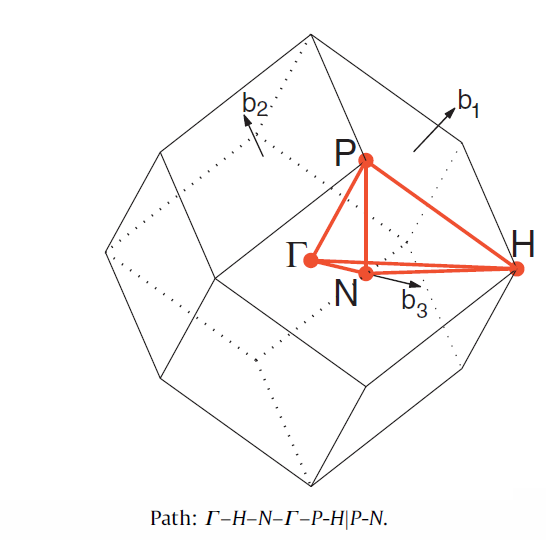
\includegraphics[height=1.0in,width=1.2in,viewport=00 0 550 520,clip]{Figures/Brillouin-Zone_BCC.png}}
%\vskip 0.10in
\subfigure[\fontsize{5.5pt}{4.2pt}\selectfont{\textrm{\ch{GeF4} band~structure}}]{
\label{Band_Gap_GeF4}
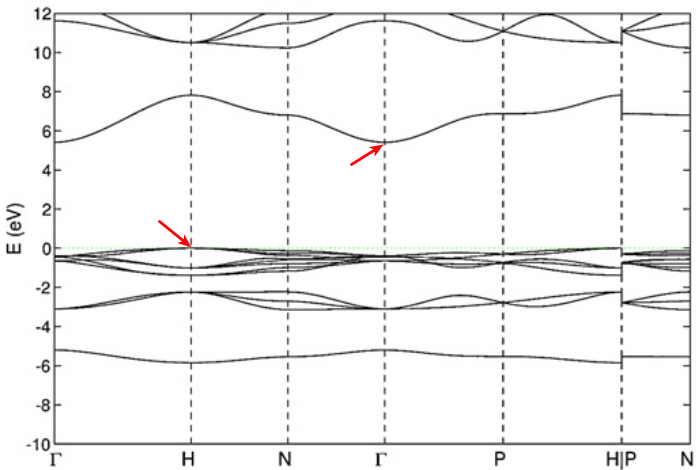
\includegraphics[height=0.8in,width=1.0in,viewport=0 0 750 500,clip]{Figures/Band-Struct_GeF4.png}}
\label{Band_Gap_BCC_GeF4}
\end{figure}
\end{minipage}
}

\frame
{
	\frametitle{$\vec k\cdot\vec p$方法加速计算}
	\begin{itemize}
		\item {\fontsize{7.5pt}{6.2pt}\selectfont{采用$\vec k\cdot\vec p$方法提升\textrm{DFT}软件的计算效率(\textrm{1-2}个数量级),计算规模增大}}
	\end{itemize}
\begin{figure}[h!]
\centering
\vskip -10pt
\subfigure[\fontsize{6.5pt}{6.2pt}\selectfont{\textrm{Band Structure}}]{
\label{band_kp}
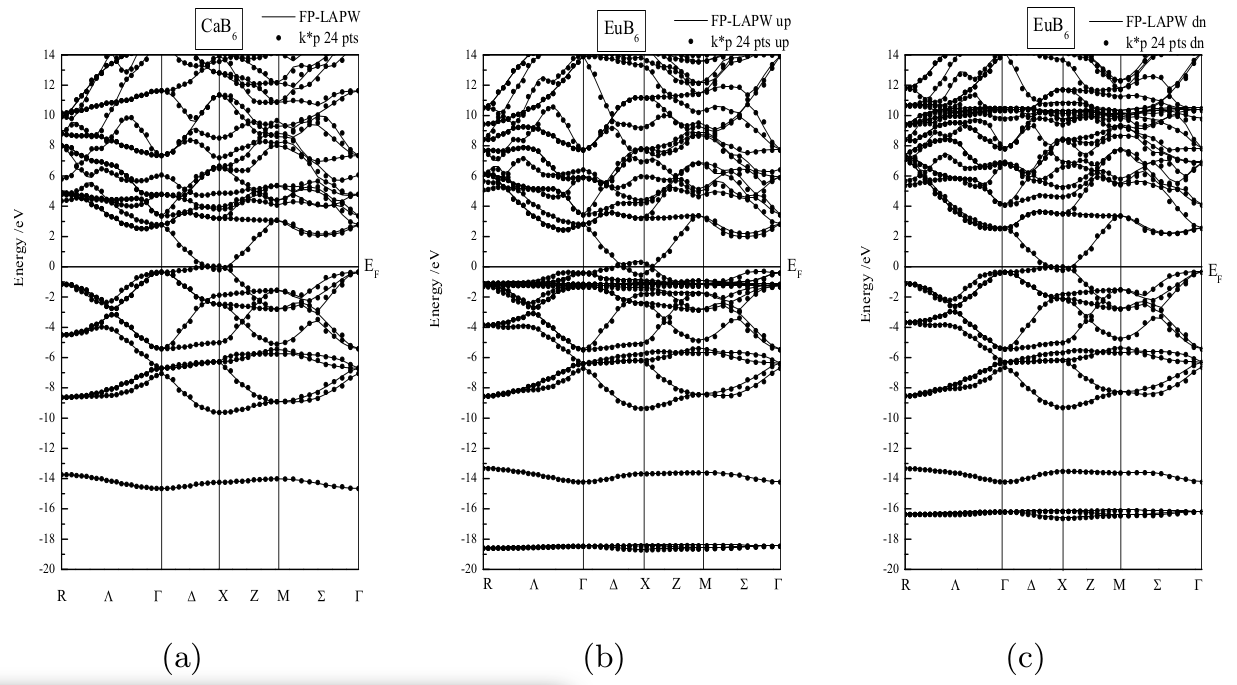
\includegraphics[height=0.9in]{Figures/Band_kp.png}}
\subfigure[\fontsize{6.5pt}{6.2pt}\selectfont{\textrm{Computing Time}}]{
\label{Time_kp}
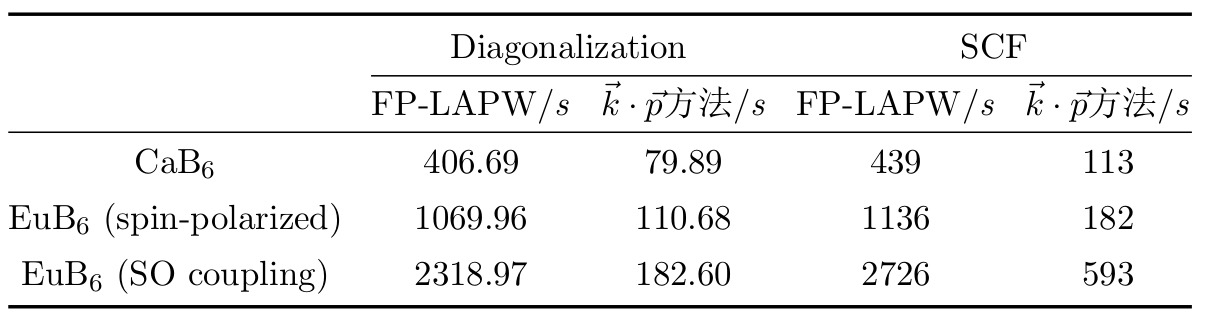
\includegraphics[height=0.6in]{Figures/Time_kp.png}}
\subfigure[\fontsize{6.5pt}{6.2pt}\selectfont{\textrm{Equation of State}}]{
\label{EOS_kp}
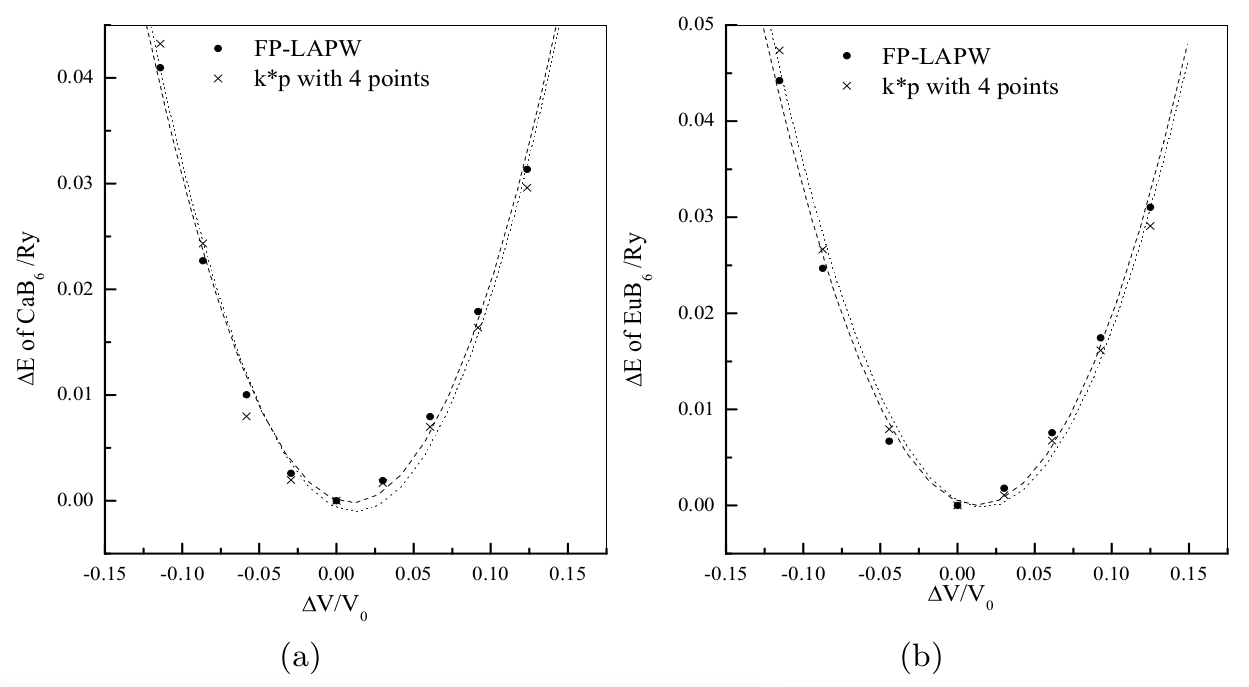
\includegraphics[height=1.0in]{Figures/EOS_kp.png}}
%\caption{\fontsize{6.2pt}{6.2pt}\selectfont{$\vec k\cdot\vec p$方法(点)与常规\textrm{DFT}方法计算的能带对比:\textrm{(a)CaB$_6$,(b)EuB$_6$-spin~up,\\(c)EuB$_6$-spin~dn}}}%
%\label{band_kp}
%\caption{\fontsize{5.2pt}{6.2pt}\selectfont{$\vec k\cdot\vec p$方法保证计算精度,并计算效率提升}}%
\end{figure}
}

%\frame
%{
%	\frametitle{\rm{DFT-MD}耦合:~复杂体系的原子相互作用势分析}
%	\begin{itemize}
%		\item \textrm{DFT}计算获得有限尺度原子间相互作用,无法支持\textrm{MD}和反应动力学的规模
%		\item \textcolor{magenta}{\textrm{DFT-MD}耦合}\\
%			机器学习方法优化\textrm{DFT}的原子相互作用,得到更精确的\textrm{MD}尺度的原子力场
%		\item 支持\textrm{MD}尺度下的材料物性模拟
%	\end{itemize}
%\begin{figure}[h!]
%\centering
%\vskip -5pt
%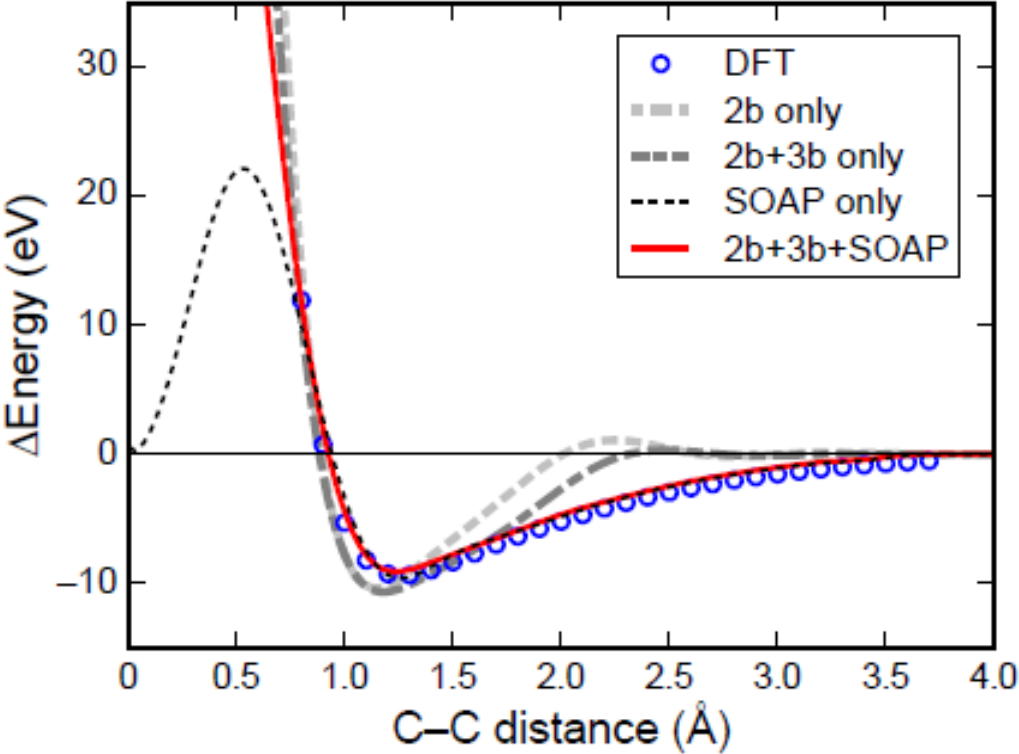
\includegraphics[height=1.2in]{Figures/poten-TiO2.png}%}
%\caption{\fontsize{7.5pt}{6.2pt}\selectfont{\textrm{ANN}优化的$\ch{TiO2}$表面的\textrm{C-C}相互作用势能面曲线,对比\textrm{DFT}结果(蓝色).}}%
%\label{ANN-poten-TiO2}
%\end{figure}
%}
%
\frame
{
	\frametitle{\rm{DFT-MD}耦合:~催化反应机理模拟流程}
\begin{enumerate}
	\item \fontsize{8.7pt}{6.2pt}\selectfont{\textrm{FireWorks}流程框架支持初始\textrm{DFT}计算并发}
	%\item 为\textrm{DFT}尺度下的原子间相互作用,启动并发式\textrm{Kohn-Sham}方程求解和化学反应动力学(反应通道)计算
	\item \fontsize{8.7pt}{6.2pt}\selectfont{筛选活化能最小的反应通道}%(\textrm{DFT-MD}尺度筛选)
%	\item \textrm{DFT}尺度下,多种结构的反应活化能计算,根据活化能确定可能的决速步
	\item \fontsize{8.7pt}{6.2pt}\selectfont{优化决速步原子间相互作用函数}%(\textrm{DFT-MD}跨尺度耦合)
	\item \fontsize{8.7pt}{6.2pt}\selectfont{求解原子的\textrm{MD}运动方程}
	\item \fontsize{8.7pt}{6.2pt}\selectfont{经\textrm{MD}模拟后确定当前体系各原子结构,返回决速步,\textrm{DFT}再次计算活化能}
	\item \fontsize{8.7pt}{6.2pt}\selectfont{迭代循环,筛选出可能的决速步,得到稳定的催化燃烧反应动力学流程,直至收敛}
\end{enumerate}
\begin{figure}[h!]
\centering
\vskip -2pt
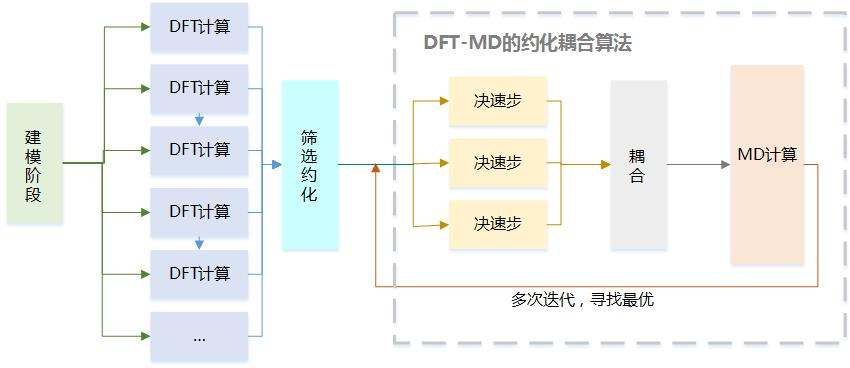
\includegraphics[height=1.05in]{Figures/CH4_complex_machine.png}
\hskip 1pt
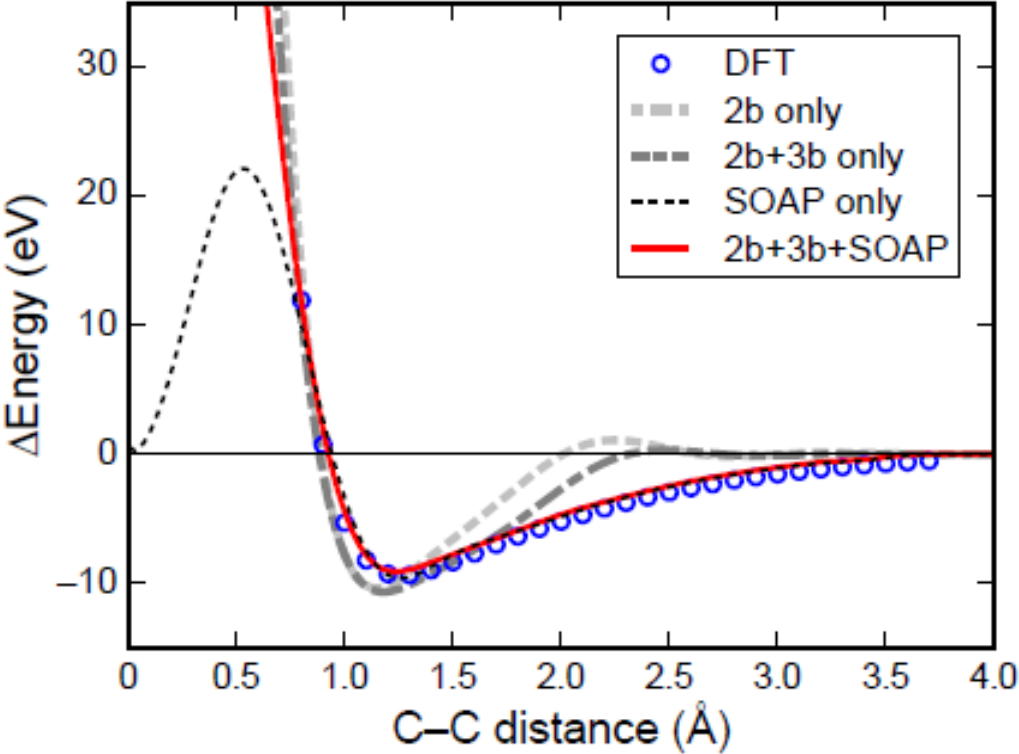
\includegraphics[height=1.05in]{Figures/poten-TiO2.png}%}
\caption{\fontsize{5.5pt}{4.2pt}\selectfont{面向催化燃烧反应动力学机理模拟的计算自动流程示意图}}%
\label{CH4_comp_BCC}
\end{figure}
}

\subsection{甲烷催化燃烧机理}
\frame
{
	\frametitle{甲烷氧化的氧交换机制}
\begin{figure}[h!]
\centering
\vskip -12pt
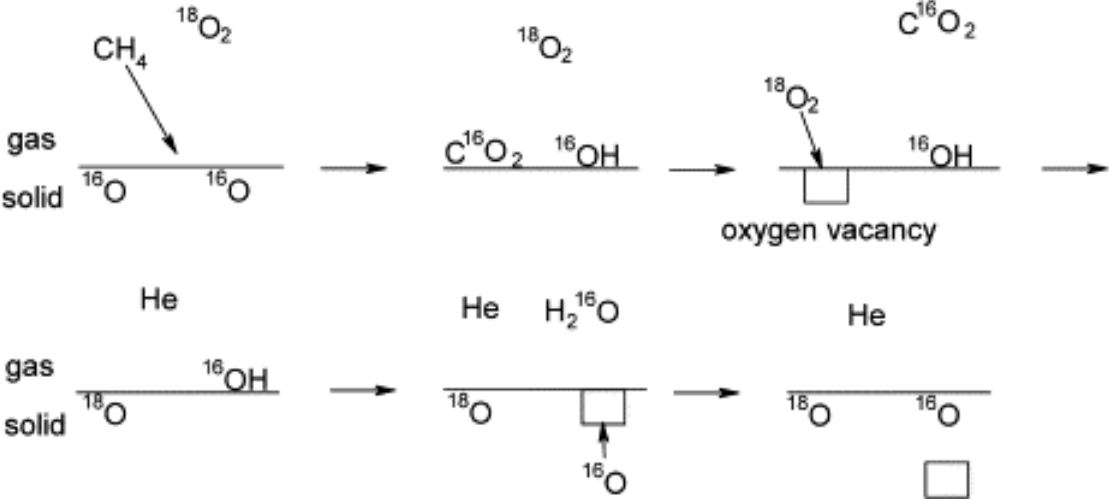
\includegraphics[height=0.8in]{Figures/Oxygen_exchange_mechanism_for_CH4_oxidation.png}
\caption{\fontsize{5.5pt}{4.2pt}\selectfont{催化剂表面甲烷氧化的氧交换过程示意}}%
\label{CH4_comp_mechan}
\end{figure}
\vskip -10pt
	{\fontsize{9.5pt}{11pt}\selectfont
\begin{displaymath}
	\begin{array}{ll}
		\mathrm{Step~1.1}\quad~&\ch{O2(g)}+{\ast}\ch{<=>}\ch{O2}^{\ast} \\
		\mathrm{Step~1.2}\quad~&\ch{O_2}^{\ast}+{\ast}\ch{<=>}2\ch{O}^{\ast} \\
		\mathrm{Step~2.1}\quad~&\ch{CH4(g)}+{\ast}+{\ast}\ch{->}\ch{CH3}^{\ast}+\ch{H}^{\ast} \\
		\mathrm{Step~2.2}\quad~&\ch{CH4(g)}+\ch{O}^{\ast}+{\ast}\ch{->}\ch{CH3}^{\ast}+\ch{OH}^{\ast} \\
		\mathrm{Step~2.3}\quad~&\ch{CH4(g)}+\ch{O}^{\ast}+\ch{O}^{\ast}\ch{->}\ch{CH3O}^{\ast}+\ch{OH}^{\ast} \\
		\mathrm{Step~3}\quad~&\ch{C}^{\ast}+\ch{O}^{\ast}\ch{<=>}\ch{CO}^{\ast}+{\ast} \\
		\mathrm{Step~4}\quad~&\ch{CO}^{\ast}+\ch{O}^{\ast}\ch{<=>}\ch{CO2}^{\ast}+{\ast} \\
		\mathrm{Step~5}\quad~&2\ch{OH}^{\ast}\ch{<=>}\ch{H2O}^{\ast}+\ch{O}^{\ast} \\
		\mathrm{Step~6}\quad~&\ch{H2O}^{\ast}\ch{<=>}\ch{H2O}+{\ast} \\
		\mathrm{Step~7}\quad~&\ch{CO2}^{\ast}\ch{<=>}\ch{CO2}+{\ast} \\
		\mathrm{Step~8}\quad~&\ch{CO}^{\ast}\ch{<=>}\ch{CO}+{\ast}
	\end{array}
\end{displaymath}}
}

\frame
{
	\frametitle{贵金属催化剂失活机制}
\begin{figure}[h!]
\centering
\vskip -12pt
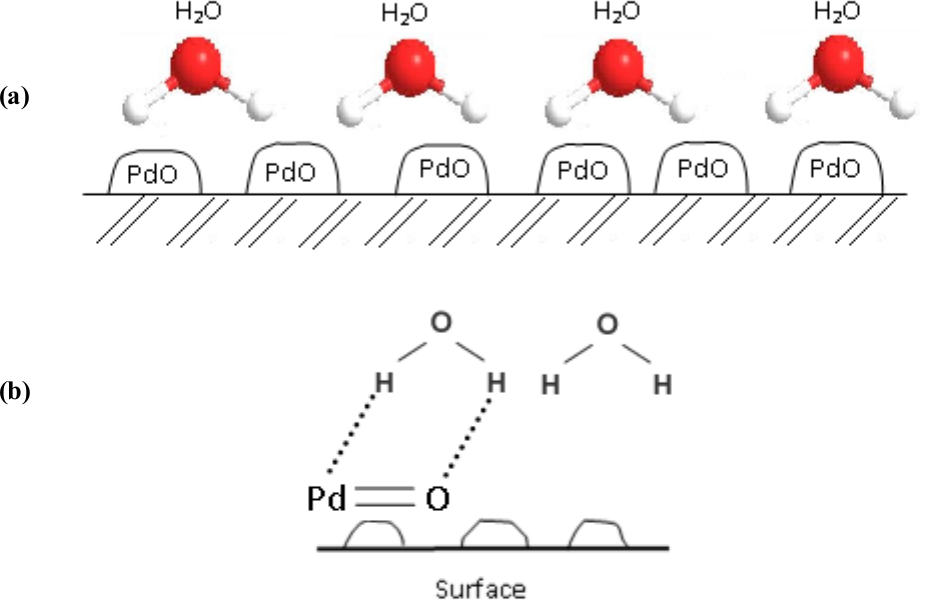
\includegraphics[height=1.2in]{Figures/PdO_H2O.png}\\
\caption{\fontsize{5.5pt}{4.2pt}\selectfont{$\mathrm{H}_2\mathrm{O}$吸附可能引起催化剂失活:~(a)$\mathrm{H}_2\mathrm{O}$吸附;(b)生成$\mathrm{Pd(OH)}_2$导致失活}}%
\label{PdO_H2O}
\end{figure}
\begin{table}[!h]
\tabcolsep 0pt \vspace*{-20pt}
%\begin{center}
\centering
\caption{\textrm{\fontsize{5.5pt}{7.2pt}\selectfont{$\mathrm{CH}_4$第一个\textrm{C-H}键断裂活化能与相应的键长、反应坐标中过渡态对应的虚频}.}}\label{Table-CH}
\vskip -12pt
\def\temptablewidth{0.92\textwidth}
\renewcommand\arraystretch{0.8} %表格宽度控制(普通表格宽度的两倍)
\rule{\temptablewidth}{1pt}
\begin{tabular*} {\temptablewidth}{@{\extracolsep{\fill}}c@{\extracolsep{\fill}}c@{\extracolsep{\fill}}c@{\extracolsep{\fill}}c@{\extracolsep{\fill}}c}
%-------------------------------------------------------------------------------------------------------------------------
	&\multicolumn{2}{c}{\fontsize{7.5pt}{7.2pt}\selectfont{$\mathrm{G}^{\neq}~(\mathrm{eV})$}}	&{\fontsize{7.5pt}{7.2pt}\selectfont{\textrm{d(C-H)}}} &{\fontsize{7.5pt}{7.2pt}\selectfont{\textrm{IMG}}} \\\cline{2-3}
	&\fontsize{7.2pt}{7.2pt}\selectfont{\textrm{PBE}} &{\fontsize{7.2pt}{7.2pt}\selectfont{\textrm{HSE}}} &{\fontsize{7.2pt}{7.2pt}\selectfont{(\textrm{\AA})}} &{\fontsize{7.2pt}{7.2pt}\selectfont{($\mathrm{cm}^{-1}$)}} \\\hline
	\fontsize{7.5pt}{7.2pt}\selectfont{{\textrm{H-ZSM-5}}} &\fontsize{7.5pt}{7.2pt}\selectfont{\textrm{2.86}} &\fontsize{7.5pt}{7.2pt}\selectfont{\textrm{2.40}} &\fontsize{7.5pt}{7.2pt}\selectfont{\textrm{1.431}} &\fontsize{7.5pt}{7.2pt}\selectfont{\textrm{1126.17}}\\
	\fontsize{7.5pt}{7.2pt}\selectfont{{$[\mathrm{AlO}_2]\mathrm{Pd}$-\textrm{H-ZSM-5}}} &\fontsize{7.5pt}{7.2pt}\selectfont{\textrm{1.39}} &\fontsize{7.5pt}{7.2pt}\selectfont{\textrm{2.00}} &\fontsize{7.5pt}{7.2pt}\selectfont{\textrm{1.686}} &\fontsize{7.5pt}{7.2pt}\selectfont{\textrm{899.81}}\\
	\fontsize{7.5pt}{7.2pt}\selectfont{{$[\mathrm{AlO}_2]\mathrm{PdOH}$-\textrm{H-ZSM-5}}} &\fontsize{7.5pt}{7.2pt}\selectfont{\textrm{1.04}} &\fontsize{7.5pt}{7.2pt}\selectfont{\textrm{1.23}} &\fontsize{7.5pt}{7.2pt}\selectfont{\textrm{1.296}} &\fontsize{7.5pt}{7.2pt}\selectfont{\textrm{812.50}}\\
	\fontsize{7.5pt}{7.2pt}\selectfont{{$[\mathrm{AlO}_2]\mathrm{Pd}(\mathrm{OH})_2$-\textrm{H-ZSM-5}}} &\fontsize{7.5pt}{7.2pt}\selectfont{\textrm{1.42}} &\fontsize{7.5pt}{7.2pt}\selectfont{\textrm{1.46}} &\fontsize{7.5pt}{7.2pt}\selectfont{\textrm{1.363}} &\fontsize{7.5pt}{7.2pt}\selectfont{\textrm{793.60}}\\
	\fontsize{7.5pt}{7.2pt}\selectfont{{$[\mathrm{AlO}_2]\mathrm{Pd}[\mathrm{AlO}_2]$-\textrm{H-ZSM-5}}} &\fontsize{7.5pt}{7.2pt}\selectfont{\textrm{2.67}} &\fontsize{7.5pt}{7.2pt}\selectfont{\textrm{2.73}} &\fontsize{7.5pt}{7.2pt}\selectfont{\textrm{1.611}} &\fontsize{7.5pt}{7.2pt}\selectfont{\textrm{683.43}}\\
\end{tabular*}
\rule{\temptablewidth}{1pt}
%\end{center}
\end{table}
}

\frame
{
	\frametitle{非金属盐催化剂活性提升}
\begin{minipage}[b]{0.32\linewidth}
\begin{figure}[h!]
\centering
\vskip 30pt
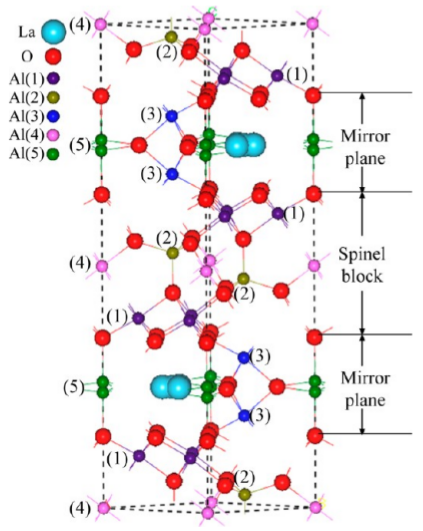
\includegraphics[height=1.62in]{Figures/MAl_12O_19_MP-type_Cat.png}\\
\caption{\fontsize{6.5pt}{4.2pt}\selectfont{\textrm{MP}型\textrm{La}-六铝酸盐.}}%
\label{MP-type}
\end{figure}
\end{minipage}
\begin{minipage}[b]{0.65\linewidth}
\begin{table}[!h]
\tabcolsep 0pt \vspace*{-85pt}
%\begin{minipage}{\0.95\textwidth}
%\begin{center}
\centering
\caption{\textrm{\fontsize{6.5pt}{4.2pt}\selectfont{六铝酸镧原胞中\textrm{Fe}离子取代位点对晶格能的影响.}}}\label{Table-MP-La}
\vskip -5pt
\def\temptablewidth{1.00\textwidth}
\renewcommand\arraystretch{0.8} %表格宽度控制(普通表格宽度的两倍)
\rule{\temptablewidth}{1pt}
\begin{tabular*} {\temptablewidth}{@{\extracolsep{\fill}}c@{\extracolsep{\fill}}c@{\extracolsep{\fill}}c@{\extracolsep{\fill}}c@{\extracolsep{\fill}}c@{\extracolsep{\fill}}c}
%-------------------------------------------------------------------------------------------------------------------------
	\fontsize{4.5pt}{4.2pt}\selectfont{\textrm{Crystal}} &\fontsize{4.5pt}{4.2pt}\selectfont{\textrm{Substituted}}	&\fontsize{4.5pt}{4.2pt}\selectfont{\textrm{Lattice-energy}} & & & \\
	\fontsize{4.5pt}{4.2pt}\selectfont{\textrm{Structure}} &\fontsize{4.5pt}{4.2pt}\selectfont{\textrm{Sites}}	&\fontsize{4.5pt}{4.2pt}\selectfont{\textrm{(eV)}} &\fontsize{4.5pt}{4.2pt}\selectfont{\textit{a}(\textrm{\AA})} &\fontsize{4.5pt}{4.2pt}\selectfont{\textit{b}(\textrm{\AA})} &\fontsize{4.5pt}{4.2pt}\selectfont{\textit{c}(\textrm{\AA})} \\\hline
	\fontsize{4.5pt}{4.2pt}\selectfont{\textrm{spinel block}} &\fontsize{4.5pt}{4.2pt}\selectfont{\textrm{Al(1)}} &\fontsize{4.5pt}{4.2pt}\selectfont{\textrm{-480.56}} &\fontsize{4.5pt}{4.2pt}\selectfont{\textrm{5.60}} &\fontsize{4.5pt}{4.2pt}\selectfont{\textrm{5.60}} &\fontsize{4.5pt}{4.2pt}\selectfont{\textrm{22.04}}\\
	&\fontsize{4.5pt}{4.2pt}\selectfont{\textrm{Al(2)}} &\fontsize{4.5pt}{4.2pt}\selectfont{\textrm{-481.49}} &\fontsize{4.5pt}{4.2pt}\selectfont{\textrm{5.60}} &\fontsize{4.5pt}{4.2pt}\selectfont{\textrm{5.60}} &\fontsize{4.5pt}{4.2pt}\selectfont{\textrm{22.05}}\\
	&\fontsize{4.5pt}{4.2pt}\selectfont{\textrm{Al(4)}} &\fontsize{4.5pt}{4.2pt}\selectfont{\textrm{-480.97}} &\fontsize{4.5pt}{4.2pt}\selectfont{\textrm{5.60}} &\fontsize{4.5pt}{4.2pt}\selectfont{\textrm{5.60}} &\fontsize{4.5pt}{4.2pt}\selectfont{\textrm{21.98}}\\
	\fontsize{4.5pt}{4.2pt}\selectfont{\textrm{mirror plane}} &\fontsize{4.5pt}{4.2pt}\selectfont{\textrm{Al(3)}} &\fontsize{4.5pt}{4.2pt}\selectfont{\textrm{-480.51}} &\fontsize{4.5pt}{4.2pt}\selectfont{\textrm{5.61}} &\fontsize{4.5pt}{4.2pt}\selectfont{\textrm{5.61}} &\fontsize{4.5pt}{4.2pt}\selectfont{\textrm{22.23}}\\
	&\fontsize{4.5pt}{4.2pt}\selectfont{\textrm{Al(5)}} &\fontsize{4.5pt}{4.2pt}\selectfont{\textrm{-480.72}} &\fontsize{4.5pt}{4.2pt}\selectfont{\textrm{5.62}} &\fontsize{4.5pt}{4.2pt}\selectfont{\textrm{5.62}} &\fontsize{4.5pt}{4.2pt}\selectfont{\textrm{22.06}}\\
	\multicolumn{3}{c}{\fontsize{4.5pt}{4.2pt}\selectfont{\textrm{initial value set for unsubstituted La-MP}}} &\fontsize{4.5pt}{4.2pt}\selectfont{\textrm{5.59}} &\fontsize{4.5pt}{4.2pt}\selectfont{\textrm{5.59}} &\fontsize{4.5pt}{4.2pt}\selectfont{\textrm{21.96}}
\end{tabular*}
\rule{\temptablewidth}{1pt}
%\end{minipage}
%\end{center}
\end{table}
\end{minipage}
}

\section{项目总结}
\frame
{
	\frametitle{应用前景}
	\begin{itemize}
		\setlength{\itemsep}{15pt}
		\item 该项目主要面向典型催化过程化学反应模拟,建立自动流程计算平台,\textcolor{magenta}{面向催化反应模拟自动流程软件};后续将流程软件可扩展到结构材料研究中,有助于提高云平台部门的材料模拟能力和范围
		\item 无论贵金属催化剂还是六铝酸盐系列催化剂等高温燃烧催化体系,此次开发的流程软件都可以用以研究催化反应机理,从理论计算角度给出合理的催化机理,为实验可控制备提供理论支持
		\item 通过现有平台的开发,推动中心在“材料基因工程”领域针对典型材料的计算流程、数据分析与可视化的科学计算平台建设
	\end{itemize}
}

\frame
{
	\frametitle{项目成果}
	\begin{itemize}
%		\setlength{\itemsep}{25pt}
		\item 第一原理催化反应模拟计算平台自动流程的技术分析报告
		\item 甲烷催化燃烧模拟的理论计算与结果分析技术报告
		\item 软件著作权2份\\
			\vskip 3pt
			\fontsize{7.5pt}{4.2pt}\selectfont{微观材料工作流可视化交互设计系统\textrm{V1.0}}\\
			\vskip 5pt
			\fontsize{7.5pt}{4.2pt}\selectfont{晶体对称性分析与电子结构标准化软件\textrm{V1.0}}
\begin{figure}[h!]
\centering
\vskip -5pt
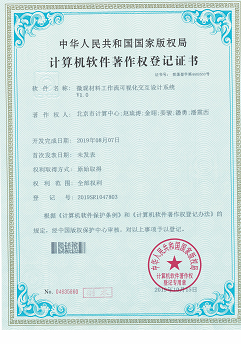
\includegraphics[height=1.82in]{Figures/Certificate-1.png}
\hskip 5pt
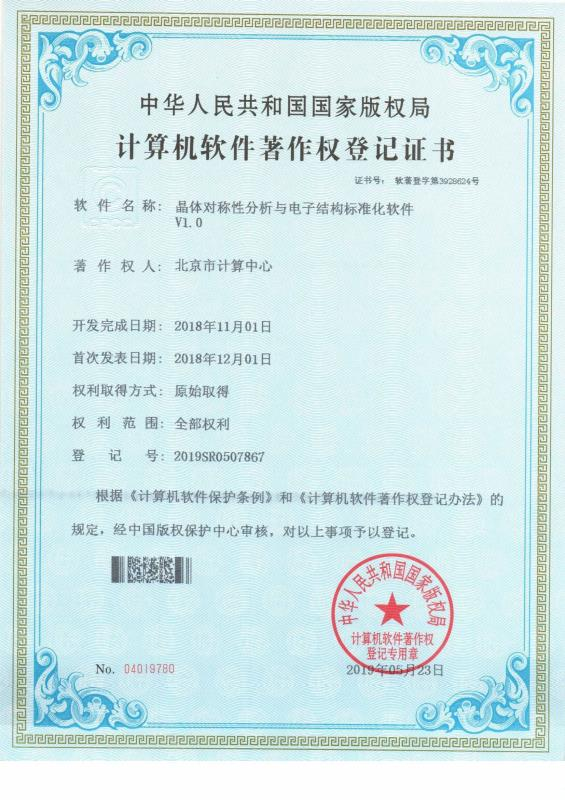
\includegraphics[height=1.82in]{Figures/Certificate-2.jpg}
%\caption{\fontsize{6.5pt}{4.2pt}\selectfont{\textrm{MP}型\textrm{La}-六铝酸盐.}}%
\label{Certificates}
\end{figure}
	\end{itemize}
}

\frame
{
	\frametitle{项目成果}
	\begin{itemize}
		\item 获奖\;\textcolor{red}{“2019中国大数据与智能计算技术创新奖”}
		\item 发表论文\\
			\vskip 3pt
			\fontsize{6.5pt}{6.2pt}\selectfont{\textrm{Y.-R. Wang, Z.-H. Du, \underline{J. Jiang}, B.-K Lu, C.-Y. Wang, Modeling the Parallel Efficiency of Density Functional Theory based Jobs on Sunway TaihuLight, IEEE CSE 2019} (最佳论文奖)}
\begin{figure}[h!]
\centering
\vskip -5pt
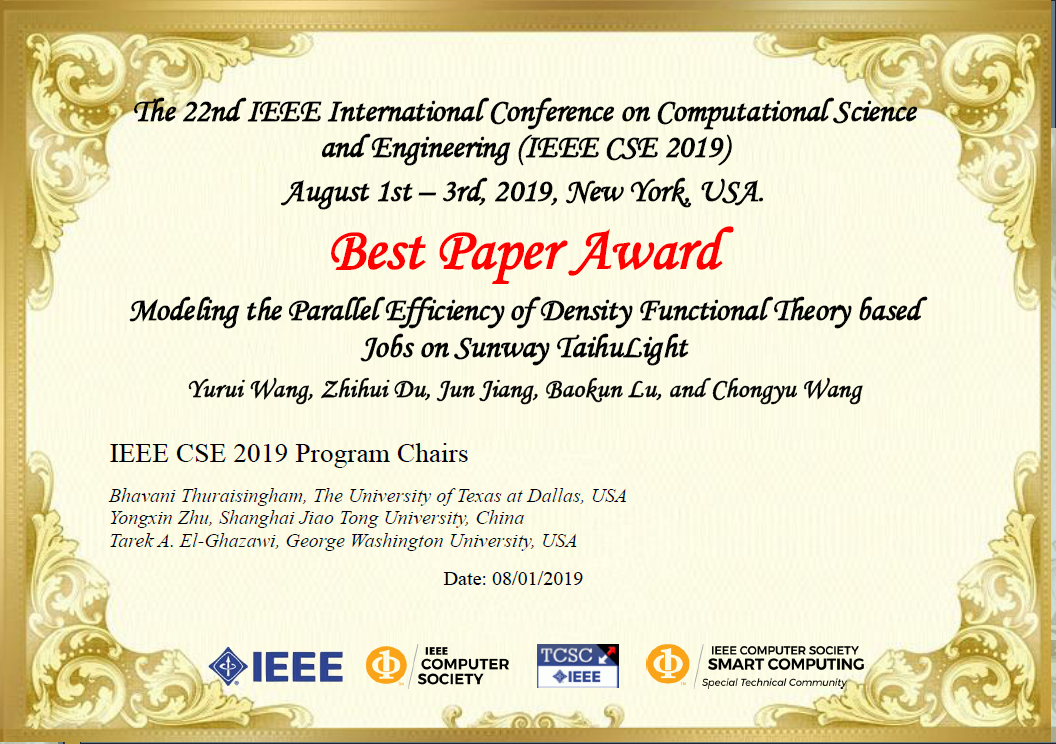
\includegraphics[height=1.02in]{Figures/Best-Paper-Wang.png}
%\caption{\fontsize{6.5pt}{4.2pt}\selectfont{\textrm{MP}型\textrm{La}-六铝酸盐.}}%
\label{Best-Paper}
\end{figure}
			\fontsize{6.5pt}{6.2pt}\selectfont{\textrm{Z.-X. Pan, Y. Pan, \underline{J. Jiang}, L.-T. Zhao, High-Throughput Electronic Band Structure Calculations for Hexaborides. In: K. Arai, R. Bhatia, S. Kapoor(eds) Intelligent Computing. CompCom. 2019, Springer, Cham 998, 386-395, (2019).}}
			\vskip 3pt
			\fontsize{6.5pt}{6.2pt}\selectfont{\textrm{Z.-H. Du, X.-N. Hui, Y.-R. Wang, \underline{J. Jiang}, J. Liu, B.-K Lu, C.-Y. Wang, Inter-Job Scheduling of High-Throughput Material Screening Applications, International Parallel and Distributed Processing Symposium (IPDPS), IEEE, 2020}}
	\end{itemize}
}

\frame
{
	\frametitle{经费使用}
	\begin{itemize}
		\item \textcolor{magenta}{经费总计:~}\textcolor{red}{5.8~}万元
	\end{itemize}
{\footnotesize{
\begin{table}[!h]
\tabcolsep 0pt \vspace*{-12pt}
\caption{经费预算表 (单位:~万元).}
\label{Table-Cost}
\begin{minipage}{\textwidth}
%\begin{center}
\centering
\def\temptablewidth{0.84\textwidth}
\renewcommand\arraystretch{1.5} %表格宽度控制(普通表格宽度的两倍)
\rule{\temptablewidth}{1pt}
\begin{tabular*} {\temptablewidth}{@{\extracolsep{\fill}}c@{\extracolsep{\fill}}c@{\extracolsep{\fill}}c@{\extracolsep{\fill}}c}
%-------------------------------------------------------------------------------------------------------------------------
	开支项目 &预算总金额	&\textrm{2018~}年度 &\textrm{2019~}年度\\\hline
设备费 &4 &2 &2\\
	差旅费 &0.5 &0.25 &0.25\\
	会议费 &0.3 &0.15 &0.15\\
	\makecell{出版/文献/信\\息传播/知识\\产权事物费} &0.2 & &0.2 \\
	专家咨询费 &0.8 &0.4 &0.4\\
\end{tabular*}
\rule{\temptablewidth}{1pt}
%\end{center}
\end{minipage}
\end{table}}}
}

\frame
{
	\frametitle{个人发展}
经过该项目的研究历程,个人得到以下能力的提升
	\begin{itemize}
		\setlength{\itemsep}{15pt}
		\item 深化对甲烷燃烧催化剂催化机理的认识,提高凝练课题目标、独立组织和完成课题任务的能力
		\item 提升在团队科研活动中人员管理、学术交流和财务分配的相关组织和业务管理能力
		\item 促进个人在材料科学计算软件开发与应用领域发现新需求的能力
	\end{itemize}
}

%\begin{thebibliography}{99}
%-----------------------------------------------------------------------------------------------------------------------------------------------------------------------%
%\frame
%{
%\frametitle{主要参考资料}
%	\bibitem{Origin-1}网络流传资料:~\textrm{Origin~}图形绘制及曲线拟合.ppt\\{\footnotesize\url{https://wenku.baidu.com/view/7e7c775de2bd960591c67705.html}}					%
%	\bibitem{Origin-2}网络流传资料:~\textrm{Origin~}图形绘制基础入门及曲线拟合.ppt\\{\footnotesize\url{https://wenku.baidu.com/view/d2b85773f46527d3240ce05e.html}}					%
%	\bibitem{Origin-3}网络流传资料:~{\textit{方东明}},~\textrm{Origin~8.0~}二维图形绘制制详解实例和教程.pdf\\{\footnotesize\url{https://wenku.baidu.com/view/eaf64026bd64783e09122b66.html}}					%
%	\bibitem{Origin-4}\textrm{Origin~}官网视频教程:\\{\footnotesize\url{http://www.originlab.com/index.aspx?go=SUPPORT/VideoTutorials}}					%
%	\bibitem{Matlab-1}网络流传资料:~\textrm{Matlab~}绘制曲线的方法.ppt\\{\footnotesize\url{https://wenku.baidu.com/view/dad6257a02768e9951e738e1.html}}					%
%\nocite*{}
%}

%\frame
%{
%\frametitle{发展统一理论框架下的材料计算程序}
%\begin{itemize}
%	\item
%\end{itemize}
%}


%-----------------------------------------------------------Beamer下不建议使用bib,因为涉及分页--------------------------------------------------------------------------%
%{\small
%\phantomsection\addcontentsline{toc}{section}{Bibliography}	 %直接调用\addcontentsline命令可能导致超链指向不准确,一般需要在之前调用一次\phantomsection命令加以修正	%
%\bibliography{Myref}																			%
%\bibliographystyle{mybib}																		%
%  \nocite{*}																				%
%}

%------------------------------------------------------------------------------------------------------------------------------------------------------------------------------%


%-------------------------------------------------------------------------Thanks------------------------------------------------------------------------------------------------
%\section{致谢}
%\frame
%{
%\frametitle{致$\quad$谢}
%\begin{itemize}
%    \setlength{\itemsep}{20pt}
%  \item 感谢本团队高兴誉、吴泉生、宋红州等各位老师参与的讨论
%  \item 感谢莫所长、宋主任以及软件中心各位老师和同事
%  \item 感谢王崇愚先生的帮助
%\end{itemize}
%}

%-------------------------------------------------------------------------------------------------------------------------------------------------------------------------------

\logo{}									%不显示logo
\frame
{
\vskip 60 pt
%\hskip 10pt \textcolor{blue}{\Huge 感谢答辩委员会各位老师\,\textrm{!}}\\
\vskip 35 pt
\hskip 60pt \textcolor{blue}{\Huge 谢谢大家\:!}
%\vskip 15 pt
%\hskip 40pt \textcolor{blue}{\Huge \textrm{for your attention\:!}}
}

%-------------------------------------------------------------------------------------------------------------------------------------------------------------------------------

\clearpage
%\end{CJK*}
\end{document}
